\documentclass[UTF8]{ctexart}
\usepackage{graphicx}
\usepackage{amsmath}
\usepackage{bibentry,natbib}
\usepackage{fancyhdr}

\title{Latent Dirichlet Allocation \\ Gibbs Sampling}
\author{BrightHush}
\date{\today}

\begin{document}
\maketitle
\tableofcontents

\pagestyle{fancy}
\cfoot{\thepage}

\newcommand{\figref}[1]{\figurename~\ref{#1}}
%\begin{figure}[h!]
%    \centering     
%    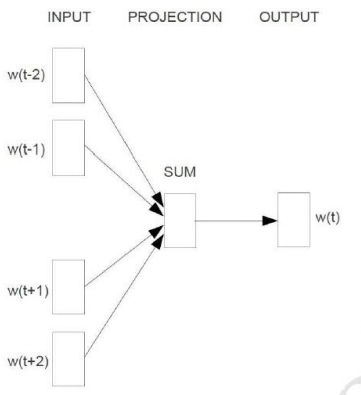
\includegraphics[width=0.5\textwidth]{cbow}   
%    \caption{\label{Fig:CBOW}CBOW Architecture} 
%\end{figure}
\section{Understanding LDA Model}
从一开始接触 Latent Dirichlet Model 到现在,时间已经很久了,陆陆续续也看了一些资料,但是发现一个问题就是
大部分资料都求全。从一开始的 MLE,到 MAP,然后到 Bayes Inference 。紧接着就是 Multinomial Distribution 
到 Dirichlet Distribution ,讲一些共轭的内容。然后又是来了 Gibbs Sampling,各种解释 MCMC 到 Gibbs Sampling
的知识。其实这一堆东西下来,读者已经精疲力竭了,哪来的力气来真正理解 LDA 建模过程的真谛。
\par
所以下面的内容经将不涉及很多数学的细节,真正还原 LDA 建模的本质,于是希望了解 Latent Dirichlet Allocation Model
数学推导细节的朋友可以跳过了。
\par
我们这样子考虑自然界的所有文本,假设其就是K个主题,每个主题下的词是按照一定分布放置的,也就是词在主题下是服从多项分布的。
注意这里的词在主题下的分布是全局的。\\
现在假如你想生成一篇文档,好了,你得先确定主题,也就是说你得给各个主题一个权重吧?于是你生成一篇文档的主题分布,当然这个
分布也是一个多项分布。假设这个文档的长度由你来确定,那么这个时候你根据这个文档目前的主题分布,依次给每个词确定一个主题。
好了这个词的主题确定了,那么你现在可以从该主题下随机产生一个词了。按照上面的过程你就生成了一篇文档了。
\par
前面我们已经提到主题下词的分布式多项分布,文档下主题的分布也是多项分布。这个时候Bayes学派的人就喜欢“作”,他说这些分布的
参数需要有一个先验,他们也不知道什么样的先验最好,于是从数学计算上考虑他们就选择了Dirichlet Distribution作为多项分布的
先验。因为Dirichlet分布和Multinomial分布共轭,两者合起来推导的后验概率也是一个共轭分布,这样两种满足这种关系的分布当然
就利于后面的公式推导和计算了。
\\
现在模型是确定了,但是现在我们只观测到了一大堆的文档,我们并不知道每个文档对应的主题分布,更不知道每篇文档下这些词分别是由
哪些主题产生的。于是我们的模型中需要推断两个关键知识:(1)每篇文档下的主题分布,对于第m篇文档的主题分布参数用$\vec{\vartheta}_m$
表示,如果有M篇文档,那么参数集合为$\theta = \{\vec{\vartheta}_m\}, m \in [1, M]$;
(2)每个主题下的词分布,对于第k个主题下的词分布我们用$\vec{\varphi}_k$表示,如果有K个主题,那么参数集合为
$\phi = \{ \vec{\varphi}_k \}, k \in [1, K]$。
\par
另外需要注意的是将 Dirichlet Distribution 选为先验分布的时候,通常使用Symmetric Dirichlet Distribution,
这就是为什么你在使用LDA开源工具的时候$(\alpha,\beta)$参数只设置了两个数值而非两个向量了。
\par
现在模型是建好了,我们如何求解模型的参数的呢?按照一些最优化的算法,我们通常是给这些参数一个随机初始化,但是我们还是不知道每篇文档下每
个词是由哪个主题生成的,于是我们现在把精力放在如何确定一个词对应主题上,也就是如果每一篇文档用$w_m$表示,那么其各词对应的
主题标号我们用$z_m$表示。这个东西我们用 Gibbs Sampling 来做,也就是如果我们知道$p(z_m|w_m)$的分布,我们就从这个分布中采样
得到$w_m$对应的$z_m$。于是按照 Gibbs Sampling 的思路,我们通常是要进行 MCMC 的链式采样,于是我们要知道$p(z_i|z_{\neg i}, w_m)$,
要计算这个呢,拆开来的话,你就要得到$p(\vec{z}_m|\vec{\alpha})$和$p(\vec{w}_m|\vec{z}_m, \vec{\beta})$,这两个
概率表达式可以通过先验和似然乘积对中间参数积分得到,拜共轭所赐,这样推导出来的形式非常简洁。那么现在假设这些“高端”的数学推导都
OK了,已经得到了$p(z_i|z_{\neg i}, w_m)$,那么就进行采样咯,就得到了文档下词对应的主题咯。
\par
由于Gibbs Sampling采样时,其到平稳分布需要多次迭代,这就是我们常说的Burn-In过程。
\par
好了,词对应主题这个隐含变量的值你都确定了,那么现在就是要从这些观测值中求我们之前设定的模型参数了。
\par
对于$\vec{\vartheta}_m$我们有$p(\vec{\vartheta}_m|\vec{z}_m,\vec{\alpha})$这个后验概率,同样是拜共轭所赐,这个后验概率
也是一个Dirichlet分布哦。
\par
对于$\vec{\varphi}_k$,我们有$p(\vec{\varphi}_k|\vec{z},\vec{w}, \vec{\beta})$,其分布的形式自然不必多说也是一个Dirichlet
分布。
\par
那么我们将分布的个变量的期望作为模型中参数的值,这样就确定了模型中各参数的值了。
\par
到这里这个模型就完事了。

\section{References}
\begin{itemize}
\item[1] Parameter estimation for text anaylysis.
\end{itemize}

\end{document}
